\vspace{-1.25em}
\section{Introduction}
\vspace{-0.5em}

The ability to use text instructions to control and interact with powerful AI models has made these models accessible and customizable for the masses. Such models include ChatGPT \citep{chatgpt}, which can respond to messages written in natural language and perform a wide array of tasks, and Stable Diffusion \citep{rombach2022ldm}, which turns natural language into an image. While those models cost anywhere from hundreds of thousands to hundreds of millions of dollars to train, there has been an equally exciting trend whereby powerful open-source foundation models like LLaMA \citep{llama} can be finetuned with surprisingly little compute and data to become instruction-following (e.g., \citep{alpaca, vicuna2023}). 

In this paper, we study whether such an approach could be applicable to sequential decision-making domains. Unlike in text and image domains, diverse data for sequential decision-making is very expensive and often does not come with a convenient “instruction” label like captions for images. We propose to instruction-tune pretrained generative models of behavior, mirroring the advancements seen in recent instruction-tuned LLMs like Alpaca \citep{alpaca}, and without relying on a large dataset of instruction-labeled trajectories.

In the past year, two foundation models for the popular open-ended video game Minecraft\texttrademark\ were released: a foundation model for behavior called VPT \citep{baker2022vpt} and a model aligning text and video clips called MineCLIP \citep{fan2022minedojo}. This has opened up an intriguing avenue to explore fine-tuning for instruction-following in the sequential decision-making domain of Minecraft. VPT was trained on 70k hours of Minecraft gameplay, so the agent already has vast knowledge about the Minecraft environment. However, just as the massive potential of LLMs was unlocked by aligning them to follow instructions, it is likely that the VPT model has the potential for general, controllable behavior if it is finetuned to follow instructions. In particular, our paper demonstrates a method for fine-tuning VPT to follow short-horizon text instructions with only \$60 of compute and around 2,000 instruction-labeled trajectory segments. 

\begin{figure}[t]
    \centering
    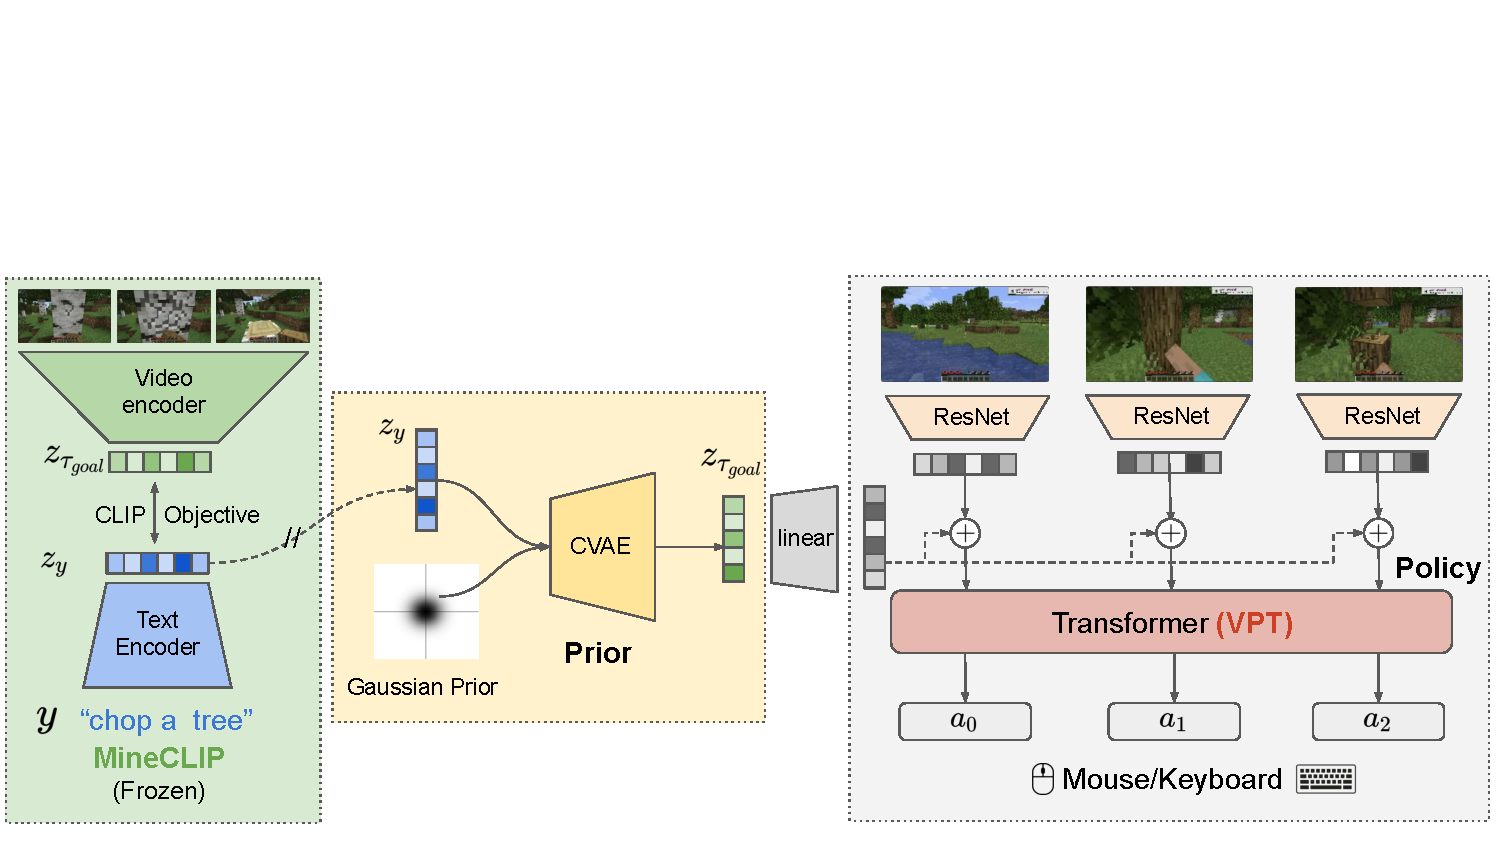
\includegraphics[width=0.9\textwidth]{figures/steve_concept.pdf}
    \caption{Like unCLIP \citep{ramesh2022dalle2}, our approach involves two models. First, we train the \textit{policy} by finetuning VPT to achieve goals given by pretrained MineCLIP \citep{fan2022minedojo} visual embeddings using our gameplay dataset. Second, for the \textit{prior} model, we train a CVAE \citep{cvae} to sample MineCLIP visual embeddings given a text prompt. The combination of these two models enables our agent to follow text and visual instructions.
    }
    \label{fig:steve_concept}
    \vspace{-1.5em}
\end{figure}

Our method draws inspiration from unCLIP \citep{ramesh2022dalle2}, the approach used to create the popular text-to-image model DALL•E 2. We decompose the problem of creating an instruction-following Minecraft agent into two models: a VPT model finetuned to achieve visual goals embedded in the MineCLIP latent space, and a prior model that translates text instructions into MineCLIP visual embeddings. We finetune VPT using behavioral cloning with self-supervised data generated with hindsight relabeling \citep{hindsight}, avoiding the use of expensive text-instruction labels in favor of visual MineCLIP embeddings. We apply unCLIP with classifier-free guidance \citep{cfg} to create our agent called \agentname{}, which sets a new bar for open-ended instruction-following in Minecraft with low-level controls (mouse and keyboard) and raw pixel inputs, far outperforming the baseline set by \citet{baker2022vpt}. 

Our main contributions are as follows:
\vspace{-0.5em}
\begin{itemize}
    \item We introduce a methodology, inspired by unCLIP \citep{ramesh2022dalle2}, for instruction-tuning generative models of behavior without relying on a large dataset of expensive instruction labels.
    \item We apply this methodology to create \agentname{}, a Minecraft agent that can follow short-horizon open-ended text and visual instructions with a high degree of accuracy, all for only \$60 of compute. We perform extensive evaluations of our agent, showing that it can robustly complete 12 of 13 goal-conditioned control tasks in our early-game evaluation suite in Minecraft. For long-horizon tasks\footnote{Short-horizon tasks require few steps: e.g., go to a tree and chop it down, dig a hole. Long-horizon tasks take many steps: e.g., craft complex recipes from scratch, build a house.} like crafting and building, we show that a basic version of prompt chaining can dramatically improve performance.

    \item We provide experimental evidence highlighting key factors for downstream performance, including pretraining, classifier-free guidance, data scaling, prompt-engineering, and other design choices. In particular, we show that unCLIP \citep{ramesh2022dalle2} and classifier-free guidance \citep{cfg} translate well to sequential decision-making and are essential for strong performance.

    \item We release model weights for \agentname{} as well as training scripts and evaluation code to help foster more research into instructable, open-ended sequential decision-making agents.\footnote{Model weights, training code, videos, and an interactive demo script are hosted on our project webpage at \href{https://sites.google.com/view/steve-1}{https://sites.google.com/view/steve-1}.}
\end{itemize}
